\section{Bayesian Analysis}

\subsection{Initial Setup - Choosing a Prior}

We start with a flat prior for the team’s win probability in Year 1, representing no initial assumptions about their performance.
This prior is expressed as a Beta(1, 1) distribution, assigning equal probability to all win rates between 0 and 1.

\subsection{Calculating Posterior for Year 1}

Using Year 1 data, we treat the number of wins as following a Binomial distribution based on the total games played.
This Binomial likelihood is combined with the Beta prior, resulting in a Beta distribution for our posterior.
The posterior for Year 1 reflects our updated belief about the team’s win probability after observing Year 1 performance.

\subsection{Updating the Prior Year-by-Year}

For each subsequent year, we treat the posterior from the previous year as the new prior.
This recursive process allows us to carry forward accumulated information, refining our estimate of the team’s win probability year after year.

\begin{figure}[!ht]
  \centering
  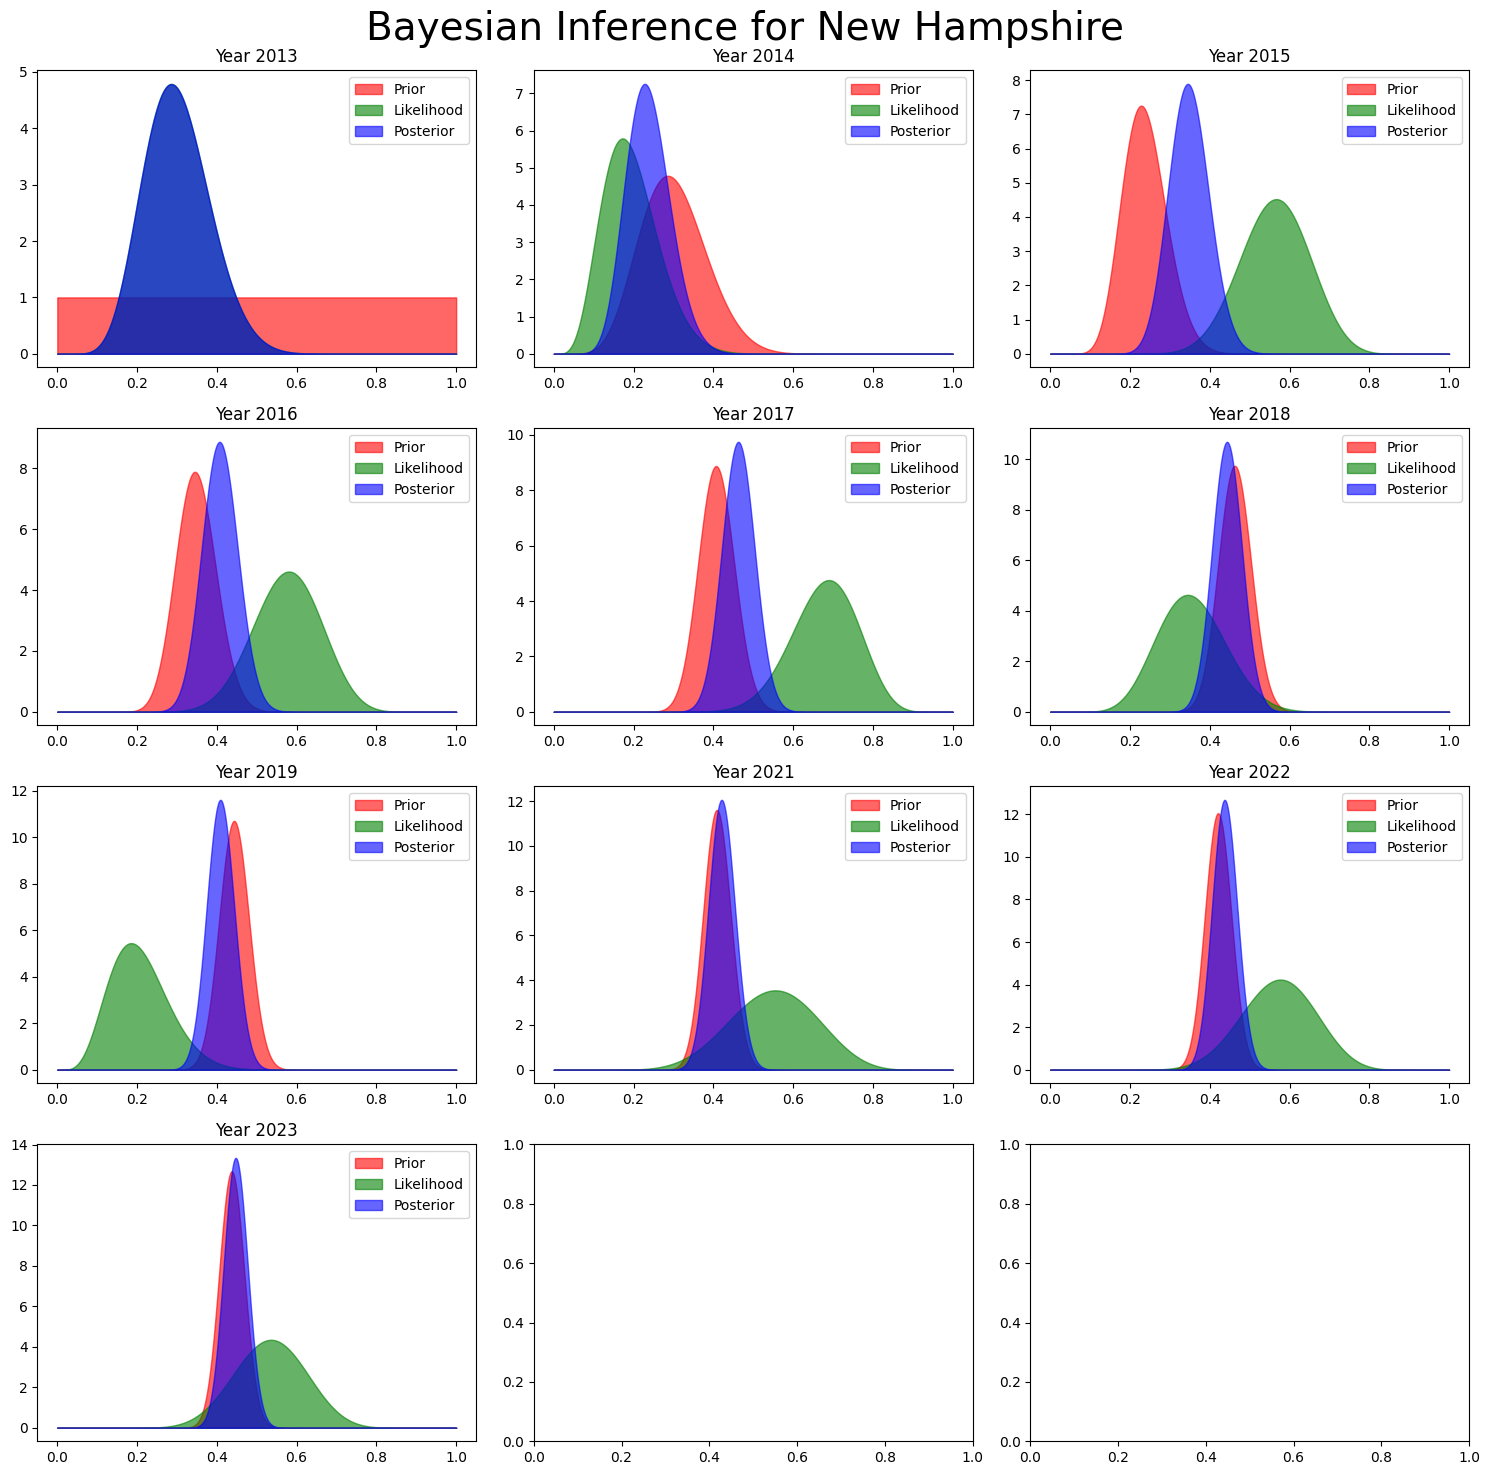
\includegraphics[width=.6\textwidth]{Project1/Report/images/posterior-subplots.png}
  \caption{Prior, Likelihood, and Posterior for each year}
\end{figure}

\subsection{Year-by-Year Posterior Distributions}

Here, we visualize the evolution of the posterior distributions over each year.
These distributions become more concentrated, indicating increased confidence as more data is incorporated over time.

\begin{figure}[!ht]
  \centering
  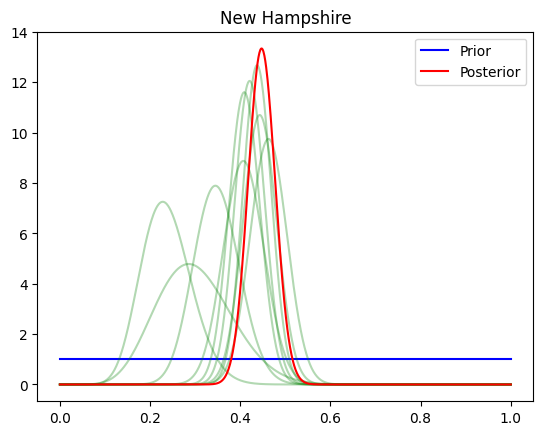
\includegraphics[width=.6\textwidth]{Project1/Report/images/posterior-years.png}
  \caption{Posterior Distributions over years}
\end{figure}

\subsection{Reporting Posterior Metrics}

By the end of 10 years, we report key metrics from the final posterior distribution.
95\% Confidence Interval: The range where the team’s win probability is most likely to lie.
Posterior Mean: The expected win probability based on all 10 years of data.
Variance: Reflects our confidence in this probability estimate; lower variance implies greater certainty.

\begin{figure}[!ht]
  \centering
  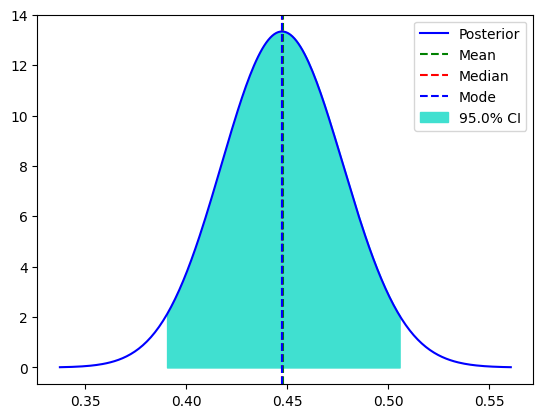
\includegraphics[width=.6\textwidth]{Project1/Report/images/confidence-interval.png}
  \caption{95\% Confidence Interval}
\end{figure}

\subsection{Posterior Mean and Variance Analysis}

The posterior mean over time shows how our estimate of win probability has evolved.
A decreasing variance suggests that our confidence is increasing, as we have more data to base our estimates on.
These metrics help us assess how consistent the team’s performance has been over time.

\begin{figure}[!ht]
  \centering
  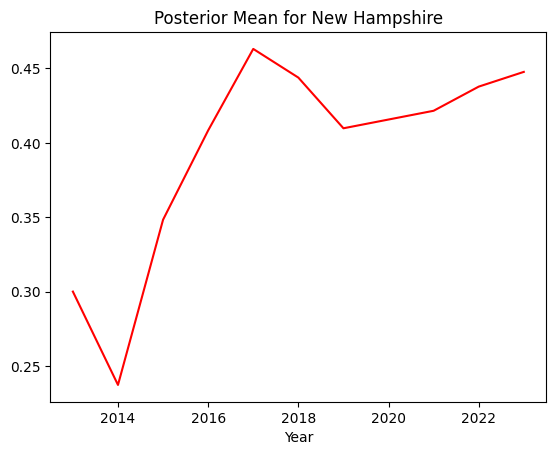
\includegraphics[width=.5\textwidth]{Project1/Report/images/posterior-mean.png}
  \caption{Posterior mean for each year}
\end{figure}

\begin{figure}[!ht]
  \centering
  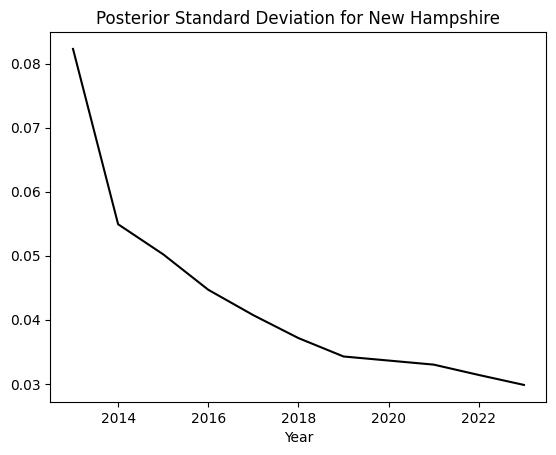
\includegraphics[width=.5\textwidth]{Project1/Report/images/posterior-sd.png}
  \caption{Posterior standard deviation for each year}
\end{figure}
